\RequirePackage[T1]{fontenc}
\documentclass[conference,10pt]{IEEEtran}
\usepackage{amsmath,amssymb,graphicx,url}
\title{Current-STA Transactional Repair for Timing--Resource Tradeoffs in 3D FPGA Routing}
\author{\IEEEauthorblockN{Anonymous development manuscript}}
\begin{document}
\maketitle
\begin{abstract}
Legal FPGA routes trade timing, wire and vertical resources. Our current-STA repair searches connection groups on private trees and commits after physical, capacity and native timing checks. Retained-crossing domains encourage sharing; search failure releases the affected network's domain. Three timing repairs improve strong native BNN from 13.607436 to 13.228146 ns for forty extra wire units. From identical fresh roots, native/domain-first flows take 7933.25/9754.31 s at equal final CPD; domain-first spends 1786 wire for 39 fewer SB/two fewer CB, attaining a fixed-terminal vertical bound. Matched owner-scope repairs escape a certified single-net local minimum with unchanged endpoint vectors. Independent feedback improves ten setup components without regressions. Fixed-input controls expose grouping, timing-budget and acceptance-scheduling tradeoffs. Robot transfer saves one CB for 20 wire; both conv-layer roles fail initial routing. Single-pass indexing preserves BNN execution at 7463.17 s. These development observations motivate broader frozen-policy confirmation.
\end{abstract}
\begin{IEEEkeywords}
3D FPGA, detailed routing, static timing analysis, transactional repair, multiobjective optimization
\end{IEEEkeywords}

\section{Problem and Motivation}
Three-dimensional FPGA routing couples directed reachability, scarce vertical channels and timing. With packing, placement and architecture fixed, repair may improve CPD or trade resources under an explicit timing requirement. Shorter local connections need not improve the complete route: another endpoint may become critical or capacity may block another network.

VTR supplies routing and timing infrastructure~\cite{vtr9paper}. Following Escaping Flatland's separation of design tradeoffs~\cite{flatland}, each comparison fixes its physical input. Reduced fixed-device occupancy does not imply silicon-area or power savings.

We use current STA to select groups, search native replacements and validate complete routes: sharing proxies alone omit timing, retained branches and convergence. 

\section{Objective and State Identity}
An input identity fixes the directed resource graph, packed netlist, placement, endpoint mapping, SDC and clock domains. A legal route $R$ uses actual graph edges and respects node capacities and native routing constraints. We record
\begin{equation}
 q(R)=(D(R),W(R),S(R),C(R),T(R)),
\end{equation}
where $D$ is native final CPD, $W$ is planar wire in the auditor's native resource units, $S$ is occupied SB pairs, $C$ is occupied CB output sources, and $T$ is comparable complete algorithm time. Paired SB half-nodes are one vertical resource; multiple CB edges from one output are not independent outputs. Guide recommendations are not occupancy measurements.

Nondominated legal candidates are retained on comparable coordinates. Four-axis quality projections preserve printed-CPD uncertainty and cannot establish five-dimensional dominance when time is unknown. Versions, convergence and repair opportunities remain explicit.

Final retention is separate from a branch's transition rule. We retain a strict CPD mode, $D(R')<D(R)$, and a fixed-resource mode that reduces CPD within registered absolute resource limits. A resource-under-timing mode permits wire tradeoffs within a fixed envelope while requiring nonincreasing selected resource objectives and at least one strict reduction. The current resource probes select $(S,C)$ as those objectives, cap CPD at the root value, cap wire at the root value plus 0.1\%, and prohibit increases beyond root vertical counts. A separate experiment fixes CPD at 102\% of the initial root once. These design parameters do not define research termination.

Endpoint-vector acceptance fixes endpoint/launch/capture identities and requires nonworse CPD, nonworse setup components, one strict setup improvement and no increased hold violation. Native comparisons use no epsilon. Resource policies apply their stated CPD/hold constraints; bounded vector additionally enforces the strict control's fixed wire/SB/CB caps. Anchors never roll forward.

\section{Mechanism: Current-State Whole Transactions}
\subsection{Select targets and dependency scopes}
Timing selection follows current native winning paths, including tied fan-ins. Capacity queries identify blocking owners; grouped targets and owner scopes release dependencies frozen by single-connection repair.

Resource selection scans the actual current route trees. A candidate removes all sinks below a selected crossing subtree, preserves paths to the other sinks, and requires both structural release potential and a retained crossing alternative. The screen uses current slack margin; it is not a proof of final resource savings. Ranking is deterministic: released crossings per removed sink, fewer sinks, larger current margin, then network and pin IDs. A K8 group contains at most eight distinct networks; fewer are used when fewer qualify. Removed connections are restored in descending current raw criticality with deterministic ties. Accepted states receive a fresh current selector.

A diagnostic selector escalates stalled source escapes. When a SOURCE's sole OPIN has unit-capacity same-layer channel exits all held by others, a same-layer sink forces an outward crossing and a distinct return resource. Owner-descendant cuts are screened by current STA and ranked by crossing excess, connection count, margins and IDs. Complete native checks still determine feasibility.

\subsection{Native searches and retained-crossing domains}
For each group we copy the selected trees and prune exactly the registered sink sets. Occupancy is updated as every local replacement is installed, so later searches see earlier resource use. Native weighted search uses the full device search box and the existing timing/congestion objective. Capacity-infeasible results are not committed. Real switch delays and final STA remain unchanged.

The domain control initially allows cross-layer edges only through crossing sources retained after pruning. It preserves useful sharing but can become infeasible under current capacities. The unrestricted native control receives the same current source, sink set, tree scope, objective and search range. Paired development probes evaluate both variants and use the registered domain-first acceptance order; native-only trajectories instead reselect from their own accepted unrestricted states. Those trajectories must not borrow a guided successor after divergence. Resource-policy execution can instead try the preferred domain candidate first and omit the optional native diagnostic only after complete resource acceptance. A rejected or infeasible domain candidate retains the same-source native fallback; omitted candidates have no inferred metrics.

If guided search fails to return a capacity-feasible branch, failure release resets search costs and removes only that network's domain. Prior restorations/occupancy remain private; other networks stay guided. Operational search failure does not certify mathematical infeasibility; a separate capacity diagnosis may establish a fixed-scope bound.

\subsection{Complete checks, acceptance and restoration}
After restoring all selected connections, independent checks validate real edges, retained branches, terminals, global capacity and resource counts; native FULL/fresh STA check the replacement. Acceptance commits the entire group; failure/rejection retains the source. Private intermediate states may spend resources/slack if the complete combination passes, allowing useful groups whose components individually fail CPD improvement.

Candidates receive native LOAD/FULL/STA, or are installed in a private worker for FULL/fresh STA and dedicated export. The latter restores trees, sink lookups, occupancy, digest and hooks before reobservation. Tiny/BNN-resource/free-path timing tests match separate same-binary LOAD/STA and physical/scope checks; large forced-path timing remains unvalidated.

Loaded contexts reset PathFinder prices; matched controls share this reset. In-router integration requires validating the price-history choice.

\section{Overall Development Results}
The implementation derives from VTR revision \texttt{0b912334fdd83bb754b302146ac0d1ec9edc9a0e}. Fixed-input serial clustered routing uses two-layer edge-encoded Hybrid-O/SB-only/CB-only graphs, ideal clocks and native FULL/STA. Each record binds physical inputs, constraints, binary, request and acceptance. Flat routing, CHANZ and general multilayer remain unvalidated. A0 is native; R1 is the older guided method. Strong BNN roots permit eight native convergence attempts with a 1.01 threshold. BNN has no supplied SDC: defaults use one ideal ap\_clk domain and zero input/output/setup/hold constraints; bound echoes fix these. U/Tf remain separate versions/opportunities.

\begin{table}[t]
\centering\caption{BNN legal quality points. Fast A0 follows three current-STA commits from pristine strong A0. Resource inputs/opportunities remain separate; both 47-SB local timing menus are terminal. Quality comparison, not matched-compute ranking.}
\label{tab:bnn}
\small
\begin{tabular}{lrrrr}\hline
State & CPD(ns) & Wire & SB & CB\\\hline
Strong A0 &13.607436&2059567&94&5062\\
Strong R1 &13.421610&2068908&86&5072\\
A0 native K8 (end) &13.607436&2059591&82&5062\\
A0 guided K8 (end) &13.607436&2061353&43&5060\\
Fast A0/native K8 &13.228146&2059603&86&5062\\
Imported native + timing &13.228146&2059627&82&5062\\
Cold native + timing &13.228146&2059631&82&5062\\
Cold guided + timing &13.228146&2061417&43&5060\\
Imported guide + timing &13.228146&2061389&43&5060\\
45 SB vector feedback &13.599798&2061253&45&5060\\
45 SB vector-rejected &13.413972&2061257&45&5060\\
R1 selective release &13.228146&2069104&72&5071\\
R1 native seed K8 &13.421610&2068956&71&5072\\
R1 guided seed K8 &13.421610&2070629&33&5071\\
Tf native seed K8 &13.421610&2074388&74&5062\\
Tf guided seed K8 &13.421610&2076038&43&5060\\
R1 joint owner scope &13.421610&2070653&32&5071\\
R1 two-pin owner &13.421610&2070657&32&5071\\
A0 guided seed K8 &13.607436&2061377&43&5060\\
Budget64 full resource &13.607436&2061423&43&5060\\
47 SB local native end &13.228146&2061249&47&5060\\
Budget64 local end &13.228146&2061076&47&5060\\\hline
\end{tabular}
\end{table}
The strong-A0 timing trajectory accepts three current-state transactions and reduces CPD by 2.787376\%, adding forty wire units with SB/CB unchanged. Its third step improves CPD but regresses a noncritical setup component, making the distinction between strict CPD and endpoint-vector policies observable. The same-source fixed-vertical policy independently selects the identical three states using exact completed-query/transaction reuse; its replay time is not evidence of speedup.

From fast A0, native K8 ends at 86 SB/2059603 wire; guided spends 279 wire for 79 SB/5061 CB. Timing after a historical 79-SB prefix reaches the timing-first/guided quality/vector with different trees, not general order commutation. Its nine-network exchange spends 1.114955 ns noncritical margin for 0.185826 ns critical gain; strict accepts, vector rejects. Source-only physical distance does not prove global native-STA optimality.

\begin{table}[t]
\centering\caption{Eltwise fixed-seed K8 controls from the same pristine A0 root, using uniform grouping and acceptance. Both branches use their own successors.}
\label{tab:eltwise}
\small
\begin{tabular}{lrrrr}\hline
State & CPD(ns) & Wire & SB & CB\\\hline
Strong A0 root &6.018101&217065&30&968\\
Native K8 &6.018101&217050&26&968\\
Paired fixed-seed K8 &6.018101&217183&24&965\\\hline
\end{tabular}
\end{table}
Eltwise guided K8 uses actual group sizes six then three. It saves one additional SB relative to the prior guided K4 endpoint, with identical CPD, wire and CB. No failure release triggers in this circuit, so the gain is attributed to grouping/domain decisions rather than fallback. The native-only branch accepts one move, then rejects three legal but resource-worse alternatives; these rejected candidates remain recorded. On SPMV, paired and native-first R1 repair produce the same legal route at 7.045986461 ns,148605 wire,zero SB and 967 CB, but remain quality-dominated by strong A0. Initial routability and a circuit-balanced timing improvement across the suite have not been established by these repair probes.

\section{Pareto Tradeoffs and Attribution}
\begin{figure*}[t]
\centering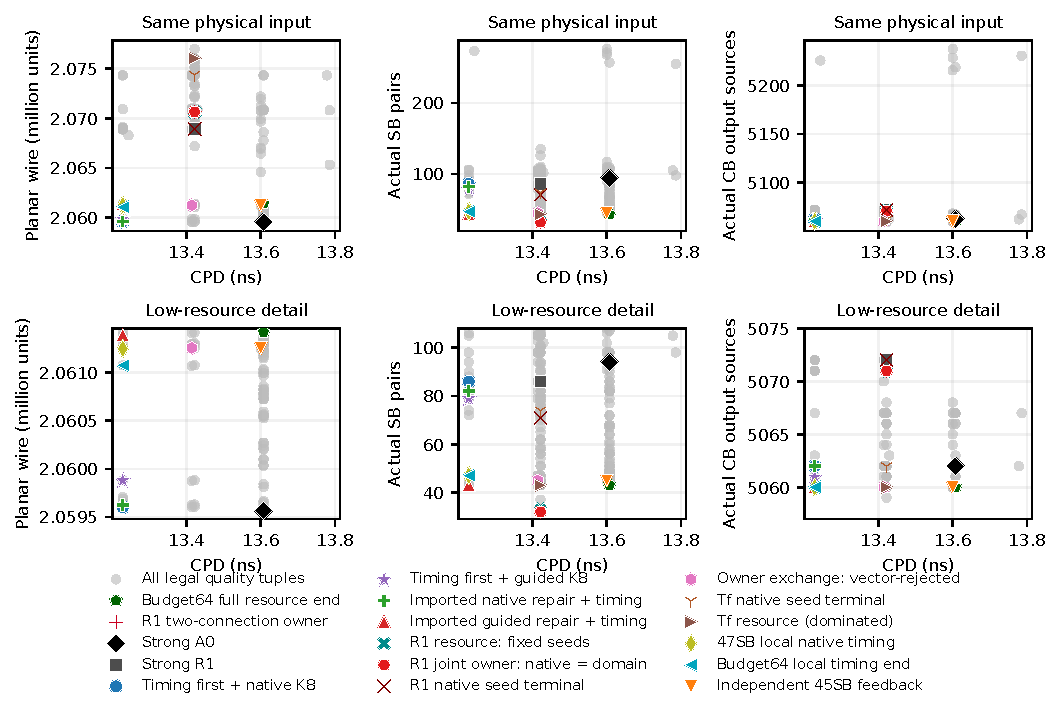
\includegraphics[width=.98\textwidth]{data/joint_quality_projection_34.pdf}
\caption{Archive 640 contains 391 BNN observations on one physical input, collapsing to 232 plotted coordinates. Both 47-SB timing menus are local terminals. Five-connection owner controls coincide; two-connection alternatives use four more wire. Budget64 full-resource and local-timing endpoints are distinct. Inputs, roots, opportunities, full vectors and costs remain in bound data; projections are not two-dimensional Pareto boundaries.}
\label{fig:joint}
\end{figure*}
Table~\ref{tab:bnn} and Fig.~\ref{fig:joint} retain external strong baselines. The fast A0 native-K8 point quality-dominates the earlier slower A0 guided-K4 point, which had the same 86 SB and 5062 CB but wire 2059667. Slower native-first low-wire states and the CB 5059 reassignment state retain distinct resource tradeoffs; the new timing prefix quality-dominates several CB 5060 predecessors. Quality domination does not establish runtime dominance with missing costs.

\subsection{Extending the native control changes the comparison}
The native-order resource cohort exhausts its current menus at 13.607436067 ns. Unrestricted native makes five commits to 2059591 wire/82 SB/5062 CB; domain-first makes nine to 2061353 wire/43 SB/5060 CB. Its 1762 extra wire buys39fewer SB/twofewerCB. Historical two-accept points are prefixes. Imported workflows 2061.28/7293.64 s create 9/19 native children; these are neither equal-compute nor cold costs.

An archived 2059567-wire/82-SB/5062-CB candidate has unchanged CPD, two setup-component improvements and none regressed. It quality-dominates the selected resource terminal; SB/CB-only acceptance rejects it. Timing continuation remains unvalidated.

Continuing from each completed resource endpoint, three strict current-STA commits reach the identical 13.228145690 ns CPD. The native branch uses 2059627 wire/82 SB/5062 CB; the paired branch uses 2061389/43/5060. The extra 1762 wire units still buy 39 SB and two CB, now at the faster timing point. Both are nondominated in the collected four-axis population and both timing menus terminate. Full-vector comparison has 550 setup improvements and 799 regressions, so equal CPD does not imply endpointwise dominance. The native imported timing phase costs 3093.90 s; the paired recovery segment costs 450.11 s, with original interrupted elapsed time unknown. Those durations are not comparable complete costs.

Fixed terminal layers require 5103 counted nonglobal networks to cross. Scanning every graph crossing verifies unit-capacity CB sources and uniquely paired unit-capacity SB halves, so distinct networks cannot share a counted resource. Thus $S+C\ge5103$, attained by 43/5060. Under $C\le5060$, $S\ge43$ is also attained. This proves fixed-graph vertical occupancy optimality, not wire, CPD or placement optimality.

A separate historical composition starts from the earlier seven-accept 45-SB/5060-CB prefix. Three strict repairs reach 13.228145690 ns at 2061301 wire/45 SB/5060 CB in 3028.24 s of imported repair. This prefix is not the final 43-SB resource input. Its full-vector branch accepts none of six proposals in 2747.93 s: one target improves physically but leaves the endpoint vector unchanged because another tied path remains; larger combinations worsen donors.

Same-source feedback drops delay-increasing donors and jointly covers two tied-path targets with three donors. The five-connection transaction reaches 13.599797732 ns (7.638334 ps gain) at 2061253 wire/45 SB/5060 CB; all ten changed setup components improve without increased hold violation. Strict/vector policies accept; imported cost is 434.52 s including preparation. A twelve-connection successor exchange reaches 13.413972155 ns at 2061257 wire: 40 fewer than the earlier equal-timing/vertical point. One setup component improves and one regresses, remaining 2.487 ns above the worst; strict accepts, vector rejects. Both orders give identical trees/vectors, costing 409.82 s excluding preparation. The controller closes thirteen proposals with only the known feedback commit and six rejected successors. Its 3755.45 s imported cost excludes initial routing and historical reuse creation.

\subsection{Automatic transfer and deterministic repair seeds}
With delay/RR-ID seeds fixed globally, eltwise native/domain roles end at 217050/217183 wire,26/24 SB,968/965 CB and 6.018101129 ns in 123.75/126.10 s of imported work. BNN A0 ends at 2059591/2061377 wire,82/43 SB,5062/5060 CB and 13.607436067 ns in 2076.31/7099.32 s. Paired wire decreases by 8 on eltwise but increases by 24 on BNN versus native-order predecessors. All eight root/control menus are closed on two circuits; roots are not independent circuit samples.

Eight fixed-seed R1 commits reduce 86 SB/5072 CB to 33 SB/5071 CB at unchanged 13.421610490 ns, adding 1721 wire to 2070629. Its 37-SB intermediate remains nondominated. At rounds 4--7, same-source unrestricted candidates fail the resource rule while guided candidates pass. The own-current native menu closes at four commits, 2068956 wire/71 SB/5072 CB at equal CPD: paired spends 1673 more wire for 38 fewer SB/one fewer CB. Native recovery takes 548.22 s; interrupted whole cost remains unknown. All eighteen legal candidates remain; 5046.61 s and nineteen native children describe imported work, not cold cost.

Tf paired makes twelve commits to 2076038 wire/43 SB/5060 CB at unchanged CPD; strong-A0's faster 43-SB point dominates it. Matched own-current native closes at eleven commits, 2074388 wire/74 SB/5062 CB. Recovery costs 1707.77 s; historical whole cost is unknown. Its rejected 2074308-wire alternative saves 80 wire at equal CPD/SB/CB but has nineteen setup improvements/four regressions; both vertical-only and endpoint-nonregression rules reject it.

Whole-four-sink repairs of R1's excess net 31767 in current-criticality/pin-ID order both save 20 wire to 2070609 with unchanged CPD/33SB/5071CB/full vector. Their different trees retain CB+SB; the vertical-only rule rejects. Shared imported cost 917.93 s excludes initial routing.

All eight same-layer OPIN exits are held by other nets. The 5104-resource state is a single-net local minimum; exact RR terminals across 78450 nets admit the 5103 reference. Original-CB-only/SB-only trials fail/restored (583.59 s imported). A prospective current-margin selector releases one blocking owner branch jointly with the target's four connections. Matched unrestricted native and target-CB-domain searches both reach 2070653 wire/32 SB/5071 CB: 24 more wire, one fewer SB, and the original CPD/full endpoint vector unchanged. Both use the same final tree; this supports owner-scope expansion, with no additional domain benefit. The aggregate 5103 attains the terminal bound. Shared two-arm imported scope costs 913.07 s, not complete or per-arm time; the original actor is unchanged. Two-connection native/retained-CB repairs and a separately constructed BFS candidate all pass FULL/STA and physical checks at 2070657 wire/32 SB/5071 CB, with the original full vector. They are dominated by the five-connection point (four fewer wire). Two-query native cores take 13.58/13.69 s versus five-query 13.40/14.19 s: fewer queries do not establish faster repair. BFS uses a different construction/LOAD binary.

\subsection{A connection budget exposes another resource tradeoff}
Complete budget64 menus preserve all 48 legal candidates (14 policy rejects). Three of four circuit/control endpoints match K8 quality. BNN guided instead ends at 2061423 wire/43 SB/5060 CB and unchanged 13.607436067 ns: 46 more wire than fixed-seed K8, with imported workflow 10568.53 versus 7099.32 s. The first four accepted rounds have identical full vectors and ordered trees. At the same fifth source, budgeting splits 77 queries into 64; final trajectories execute the same 2722-query multiset but 32 versus 18 transactions, repeating loading/audits. Smaller per-scope groups need not reduce total work. These are development imported costs, not cold or statistical speedups.

Budget64 preserves whole cuts and falls back to the first oversized cut if none fits. A separate same-source 48-SB probe selects 54 connections instead of 462. ON reaches 2061036 wire/47 SB/5060 CB at unchanged CPD, with 57 setup improvements/24 regressions and no increased hold violation; resource acceptance passes, vector rejects. It saves 177 wire versus native 47-SB/2061213 wire; guided 45-SB/2061285 wire remains a tradeoff. Core costs 51.31/60.11 s versus historical 509.71/476.90 s and shared imported-scope 948.00 s exclude initial routing and are not full-flow speedups.

From the same guided 48-SB source, unrestricted 462-connection and budget64 guided 54-connection alternatives both complete three current-STA commits under the original 2061627-wire/47-SB/5060-CB envelope. Both end at 13.228145690 ns, but guided uses 2061076 wire versus native 2061249: 173 fewer at identical vertical counts, dominating this local control. Against the complete 43-SB point it saves 313 wire for four more SB. Guided's 13.413972155-ns/2061072-wire intermediate remains a tradeoff.

All three timing requests, connection-delay changes and endpoint changes match. The first replacement's complete physical trees agree, preserving 177 wire; later trees differ, shrinking that advantage to 173. These are different full source states, not byte-equivalent trajectories or one-factor domain/grouping isolation. Actual complete timing segments cost native/guided 3056.67/3008.02 s, with source reobservation 210.01/210.48 s separately. Resource-prefix creation, query-graph preprocessing and initial routing are excluded; neither is a pristine whole-native trajectory or cold complete algorithm result.

\subsection{Capacity feedback changes the domain decision}
An all-eight-domain R1 transaction fails at network 31767/pin 1 after five successful restorations. A directed path exists when occupancy is ignored. Under the recorded transient occupancy, the retained domain has no capacity path while an unrestricted witness exists. Reconstructing the minimum occupancy immediately after pruning also leaves no domain-capacity path. Because subsequent restorations only add occupancy, changing order or search pressure cannot fix this particular frozen scope/domain. The diagnostic searches a relaxed superset of native re-expansion/closure choices; its negative result is a necessary infeasibility certificate for that scope, not for the entire FPGA.

Releasing only that network's domain yields a fully legal state at 72 SB, compared with 74 SB for the same-source unrestricted control, at the cost of 64 wire units and unchanged CPD/CB. The automatic native release implementation obtains exactly the prior selective-domain route and full endpoint vectors without a manually supplied release network or restarting earlier restorations. Nine setup components improve and none regress, so endpoint-vector acceptance succeeds while strict CPD rejects. All 23 components in a fixed source near-critical band stay unchanged. This step demonstrates resource and secondary-timing benefit, not later CPD improvement.

\subsection{Grouping contribution}
Fast-A0 native K8 matches two K4 steps in routes/vectors. Its first K4 component is endpoint-flat/rejected; K8 improves one setup component without regressions, supporting whole combinations, not a pristine-root endpoint trajectory.

\section{Overhead, Limitations and Next Confirmation}
Table~\ref{tab:completecost} binds full configurations from supplied RR graph, architecture, BLIF and packing/placement through indexes, fresh routing and complete repair. Small-circuit flows use one bound binary; BNN binds distinct resource, native-repair and candidate-STA binaries. Eltwise native accepts once/four scopes, domain-first twice/two; pairing spends 133 wire for two fewer SB/three fewer CB, with 31 less wire than native traversal.
\begin{table}[t]
\centering\footnotesize\setlength{\tabcolsep}{3pt}
\caption{Complete serial configurations. N/D: native-only/domain-first. Repair seeds: delay/RR-ID except $^\dagger$native traversal. Fused/snapshot/lazy are domain-first variants. Alternate-topology rows use eltwise; others Hybrid-O. Router seed11; SB102\% fixes CPD at 1.02 times the root. PSS: sampled tree sum in GiB.}
\label{tab:completecost}
\begin{tabular}{lrrrr}\hline
Circuit/role & CPD(ns) & Wire/SB/CB & Time(s) & PSS\\\hline
Eltwise N&6.018101&217050/26/968&290.19&1.274\\
Eltwise D&6.018101&217183/24/965&289.21&1.302\\
Eltwise D$^\dagger$&6.018101&217214/24/965&289.66&1.297\\
SPMV N&7.034698&148463/0/967&91.69&1.010\\
SPMV D&7.034698&148463/0/967&91.55&1.034\\
Softmax N&8.975747&169486/3/713&274.22&2.502\\
Softmax D&8.975747&169486/3/713&336.68&2.534\\
Eltwise fused&6.018101&217183/24/965&313.74&1.296\\
Eltwise lazy&6.018101&217183/24/965&203.48&1.310\\
SB-only N&6.040485&227439/999/0&424.59&1.271\\
SB-only D&6.040485&227459/999/0&533.57&1.282\\
CB-only N&5.862299&212511/0/982&74.15&0.740\\
CB-only D&5.862299&212511/0/982&72.46&0.740\\
Eltwise snapshot&6.018101&217183/24/965&280.37&1.300\\
SB 102\% N&6.040485&227439/999/0&448.09&1.285\\
SB 102\% D&6.114032&227583/995/0&581.65&1.257\\
BNN cold N&13.228146&2059631/82/5062&7933.25&11.055\\
BNN cold D&13.228146&2061417/43/5060&9754.31&11.063\\
BNN index N&13.228146&2059631/82/5062&7463.17&11.062\\
Robot N&13.354624&251116/9/653&377.71&2.517\\
Robot D&13.354624&251136/9/652&424.45&2.509\\\hline
\end{tabular}
\end{table}

Known-circuit transfer adds four roles: robot native/domain reach 251116/251136 wire, 9/9 SB and 653/652 CB at equal 13.354624073 ns. Domain spends 20 wire and 46.74 s for one CB. The first same-source transaction saves CB on still-guided net3140 while two other nets release failed domains; this is a combined treatment, not isolated release attribution. Both conv-layer roles fail initial routing within 200 iterations, costing 260.10/254.57 s; neither tests repair or contributes legal quality. Thus two of four roles succeed, without an unseen-test claim.

Both SPMV roles retain 148463 wire/0 SB/967 CB with no eligible cut or repair; this is not global optimality. Both softmax controls reduce 6 to 3 SB and 169490 to 169486 wire at unchanged 8.975747257 ns/713 CB. Domain-first adds one native transaction and 62.46 s without quality gain. No search-failure release occurs in these circuits or eltwise; universal domain gains are unsupported.

Fused FULL/STA preserves four candidate vectors, trees, decisions and quality but takes 313.74 s versus 289.21 s for separate LOAD/STA; source controls cost 41.90 s. In-call snapshots remove controls with unchanged four calls/64 queries/101 attempts, taking 280.37 s. All actual requests and states match; PSS 1.300 GiB has three missing reads. Fewer processes alone do not establish speedup.

Acceptance-ordered execution instead computes ON first and skips two OFF diagnostics only after legal resource acceptance. Every executed candidate and selected state matches exactly; queries fall from 64 to 32 and attempts from 101 to 51. Complete elapsed time is 203.48 s, 85.74 s (29.65\%) less in this observation. Skipped outputs are not imputed. The fixed schedule transfers to softmax with exact executed states: 271.70 versus 336.68 s, skipping one OFF. SPMV has no eligible cut or skipped work and takes 93.15 versus 91.55 s. These are single development observations, not statistical speedups.

Topology transfer fixes eltwise packing/placement and the audited n40/w100 plane. SB-only native/domain reduce 1012 to 999 SB at unchanged 6.040485445 ns; domain spends 20 more wire and 108.98 s. The 996-SB ON candidate exceeds the CPD cap, so actual OFF fallback retains 999 SB. This is post-STA policy fallback, not search-failure release. CB-only has no eligible cut: 982 cross-layer nets require 982 distinct unit-capacity OPIN sources, attaining the vertical lower bound, not wire/CPD optimality. Separately fixing CPD at 102\% of the root (6.161295154 ns) accepts the ON tradeoff; subsequent OFF reaches 995 SB. Native/domain end at 227439/227583 wire and 6.040485/6.114032 ns in 448.09/581.65 s. Domain spends 144 wire, 1.218\% CPD and 133.56 s for four fewer SB. This development-derived fixed budget never rolls and is not held-out confirmation.

Router seed11-to19 repeats all four eltwise/softmax initial/final trees, vectors, executed candidates and decisions exactly; these add no independent routing-root or circuit samples.

Fresh BNN roots match exactly. Domain-first makes nine resource commits versus five; both make three timing commits. Equal CPD costs 1786 wire and 1821.07 s for 39 fewer SB/two fewer CB, with 534 setup improvements/803 regressions and no increased hold violation. Older imported N/D points have four/28 fewer wire but unknown complete costs. Native wrappers, candidate LOAD/FULL/STA, selection and indexes dominate complete cost; detailed disjoint timings and nested cores are separately bound. All actual checks/rejections/restoration/seals are timed. Six timing audits per case consume legacy metadata aliases byte-identical to generated indexes; these remain static dependencies, without route/candidate/query history. Half-second PSS has 30/26 missing reads. The 640-record archive preserves 26 successful complete configurations on 5 known circuits/3 vertical families; later engineering batches remain separately bound. Packing/placement generation is upstream; shared-host/OS-cache effects preclude statistical speedup claims.

Jointly generating the three graph indexes in one traversal preserves all payloads and actual downstream states, requests and native work. The complete BNN command takes 7463.17 versus 7933.25 s: 470.07 s (5.93\%) less in this single shared-host observation, at identical final quality. PSS is 11.062 GiB with 21 missing reads. This uses actual full commands, not a component-time splice; legacy static metadata dependencies remain.

Timing gains concentrate in BNN; resource transfer does not establish initial routability. K1/K4/K8 and scheduling pilots remain distinct. Confirmation must freeze rules, extend circuits/seeds/architectures, and match A0/R1/native scope, targets, domains and acceptance opportunities; pooled complete time remains unknown.

\subsection{Validation overhead}
Four roles/two circuits preserve all thirty-four legal candidates, including rejects, in full vectors, ordered routes, requests/domains and decisions across legacy/direct/native-count implementations. Six transactions/six corruption guards pass. Native counters match independent references but remain native assurance, with separate final audits/context seals. Supplementary receipts retain imported validation costs; pooled complete costs remain unknown. Binary32 tree accumulation reproduces all 230693 native R1 sink delays; physical switch sums never substitute for endpoint STA.

Reproduce from source/input bindings in \path{multiobjective_connection_budget_closed_01/completion.json}; its archive preserves all 640 observations, including dominated and failed-policy legal candidates. Projection/feedback receipts distinguish final states, interrupted costs and historical prefixes.

\section{Conclusion}
Complete 43 SB/5060 CB repair attains the fixed-terminal vertical bound, spending 1786 wire and 1821.07 s for 39 fewer SB/two fewer CB at equal CPD; Matched native/domain owner-scope repairs reach 32 SB with unchanged endpoint vectors, escaping a certified single-net local minimum. Tied-path feedback and acceptance-ordered execution preserve distinct benefits. Robot transfer exposes a CB/wire/cost tradeoff and conv-layer failure limits applicability. Single-pass indexing preserves BNN quality and work with lower observed whole cost. Budget fragmentation shows why local query reductions need complete-trajectory tests. Broader frozen-policy and pooled-runtime confirmation remain required.

\begin{thebibliography}{2}
\bibitem{vtr9paper} M. A. Elgammal et al., ``VTR 9: Open-source CAD for fabric and beyond FPGA architecture exploration,'' \emph{ACM Trans. Reconfigurable Technol. Syst.}, 2025, doi:10.1145/3734798.
\bibitem{flatland} C. Hao, A. B. Kahng, B. Pramanik, and I. Youssef, ``Escaping Flatland: A placement flow for enabling 3D FPGAs,'' in \emph{Proc. ACM/IEEE DAC}, 2026, doi:10.1145/3770743.3804424.
\end{thebibliography}
\end{document}
